\documentclass[12pt, a4paper, openany]{memoir}
\usepackage[top=2.5cm, bottom=2.5cm, left=2.5cm, right=2.5cm]{geometry}
\usepackage{listings}
\usepackage{color}
\definecolor{deepblue}{rgb}{0,0,0.5}
\definecolor{deepred}{rgb}{0.6,0,0}
\definecolor{deepgreen}{rgb}{0,0.5,0}
% Default fixed font does not support bold face
\DeclareFixedFont{\ttb}{T1}{txtt}{bx}{n}{8} % for bold
\DeclareFixedFont{\ttm}{T1}{txtt}{m}{n}{8}  % for normal
\usepackage{algorithm2e}
\usepackage[noend]{algpseudocode}
%\usepackage{algpseudocode}
\usepackage{graphicx}
\usepackage[none]{hyphenat}
\usepackage{csvsimple}
%\usepackage{placeins}
\usepackage{chngcntr}
\usepackage{amsmath} %matrix
\usepackage{indentfirst} %indent the first paragraph after new section
%\usepackage[style=authoryear]{biblatex}
\usepackage{tikz} % flowchart
\usetikzlibrary{shapes,arrows} % flowchart
\usepackage{hyperref} % links
\usepackage{subcaption}
\usepackage[section,above,below]{placeins} % floatbarrier em tudo?
\usepackage{listings}
%\usepackage{fancyhdr}
%\pagestyle{fancy} 
%\fancyhf{}

\setsecnumdepth{subsection} %show number in subsection
\maxtocdepth{subsection} %show subsection in toc

\tikzstyle{decision} = [diamond, draw, fill=blue!20, 
text width=4.5em, text badly centered, node distance=3cm, inner sep=0pt]
\tikzstyle{block} = [rectangle, draw, fill=blue!20, 
text width=5em, text centered, rounded corners, minimum height=4em]
\tikzstyle{line} = [draw, -latex']
\tikzstyle{cloud} = [draw, ellipse,fill=red!20, node distance=3cm,
minimum height=2em]


\newcommand{\norm}[1]{\left\lVert#1\right\rVert}


\title{ \normalsize \textsc{Master 1 - Final year project}
	\\ [2.0cm]
	\hrule
	\vspace{0.5cm}
	\LARGE \textbf{\uppercase{Vortex detection and fitting in turbulent flows}} \\ [0.5cm]
	\hrule
	\vspace{0.5cm}
	\normalsize  \vspace*{5\baselineskip}}


\date{\vfill June - 2017}

\author{
	\Large Guilherme Lindner \\ [1.0cm]
	Research Advisors: \\
	Jean Marc Foucaut \\
	Jean-Philippe Laval  \\ [1.0cm]
	International Master on Turbulence\\ [0.2cm]
	Ecole Centrale, Lille \\}

\begin{document}
	
	\maketitle
	\thispagestyle{empty}
	\let\cleardoublepage\clearpage
	\frontmatter
	\begin{abstract}
		In this project, a tool is developed in Python to detect and evaluate the vortices of a velocity field from both numerical and experimental data. The workflow is from the thesis of Sophie Herpin \cite{herpin2009}, 2009.
		This tool comprehends the reading of NetCDF files and applying a method for detecting the vortices, like swirling strength of Q criterion. After this, all the vortices found are fitted to the Lamb-Oseen vortex using a non-linear least squares method and the correlation between the model and original data is evaluated. If the correlation is higher than 0.75, the vortex is accepted, otherwise is reject.
	\end{abstract}
	\newpage
	\tableofcontents
	\newpage
%	\thispagestyle{empty}
	\listoftables
	\newpage
	\listoffigures

    \mainmatter

\chapter*{Introduction}
\addcontentsline{toc}{chapter}{Introduction} %\markboth{INTRODUCTION}{}
Coherent structures and vortices sometimes are misunderstood for not having a clear definition. In general ways, any form of pattern arising in the flow that has an effect on it is considered a coherent structure. Meanwhile, the vortices are commonly explained as the existence of some kind of rotation in the flow. The difficulty on identifying these vortices it's in the fact that is not so clear to measure the extension of the vortex from its center of rotation. All of this becomes more complicated when we have the interaction between multiples coherent structures. According to Shawn \textit{et al} (2005) \cite{shawn2005} the definition is:
\begin{quote}
	\textit{"It is generally accepted that flows with general time dependence admit emergent patterns which influence the transport of tracers, those structures are often generically refered to as Coherent Structures"}
\end{quote}

In short we can say that vortices are one of the specific definition for coherent structures.



\chapter{Methodology}

The methodology used in this work to characterize the coherent structures are divided in three main steps: the calculation of a local function to detect the vortex; the localization of the maxima of this function; and the adjustment (fitting) of this field to the proposed model.

\section{Detection methods}
In this section, the detection methods implemented in the code for vortex identification are presented. These methods are based on the velocity gradient tensor, $\overline{D}$, that can be written as:

\begin{equation}
D_{ij} = \frac{\partial u_i}{\partial x_j}
\end{equation}

As this is a second order tensor, it can be decomposed into a symmetric and anti-symmetric part, $D_{ij} = S_{ij} + \Omega_{ij}$ where:

\begin{equation}
S_{ij} = \frac{1}{2} \left(\frac{\partial u_i}{\partial x_j} + \frac{\partial u_j}{\partial x_i}\right)
\end{equation}

\begin{equation}
\Omega_{ij} = \frac{1}{2} \left(\frac{\partial u_i}{\partial x_j} - \frac{\partial u_j}{\partial x_i}\right)
\end{equation}
$S_{ij}$ is known as the rate-of-strain tensor and $\Omega_{ij}$ is the vorticity tensor.

The characteristic equation for $\nabla u$ is given by

\begin{equation}
\lambda^3 + P \lambda^2 + Q \lambda + R = 0
\end{equation}
where P, Q and R are the three invariants of the velocity gradient tensor. Using the decomposition into symmetric and anti-symmetric parts, these invariants can be expressed as:
\begin{equation}
P = -tr(\bar{D})
\end{equation}

\begin{equation}
Q = \frac{1}{2} (tr(\bar{D})^2 -tr(\bar{D}^2)) = \frac{1}{2} (\norm{\Omega}^2 - \norm{S}^2)
\end{equation}

\begin{equation}
R = -det(\bar{D})
\end{equation}

\subsection{Q criterion}

The Q criterion proposed by Hung \textit{et al} (1988) identifies the vortices as flow regions with positive second invariant of $\nabla u$. An additional condition is that the pressure in the eddy region should to be lower than the ambient pressure. Chakraborty \textit{et al}(2005) \cite{chakra2005} quoted "in an incompressible flow Q is a local measure of the excess rotation rate relative to the strain rate".

In practical terms, the vortex is detected in case of the second invariant $Q > 0$.

\subsection{$\Delta$ criterion}

Chong \textit{et al} (1990) \cite{chong1990} define a vortex core to be the region where $\nabla v$ has complex eigenvalues. In order to determine if the eigenvalues are complex, we examine the discriminant of the characteristic equation, considering the flow incompressible (P = 0).

\begin{equation}
\Delta = \left(\frac{Q}{3}\right)^3 + \left(\frac{R}{2}\right)^2 > 0
\end{equation}


\subsection{Swirling strength criterion}

The swirling strength criterion ($\lambda_{ci}$) was developed by Zhou \textit{et al} (1999) \cite{zhou1999}. It defines a vortex core to be the region where $\nabla v$ has complex eigenvalues. It is based on the idea that the velocity gradient tensor in Cartesian coordinates can be decomposed as:

\begin{equation}
\nabla u = [\bar{\nu_r} \bar{\nu_{cr}} \bar{\nu_{ci}}]^T
\left[\begin{array}{ccc}
\lambda_r & 0 & 0 \\
0 & \lambda_{cr} & \lambda{ci} \\
0 & -\lambda{ci} & \lambda{cr} \end{array}\right]
[\bar{\nu_r} \bar{\nu_{cr}} \bar{\nu_{ci}}]^T
\end{equation} 
where $\lambda_r$ is the real eigenvalue, related to the eigenvector $\bar{\nu_r}$, and the complex conjugate pair of complex eigenvalues is $\lambda_{cr}  \pm i\lambda_{ci}$, related to the eigenvectors $\bar{\nu_r} \pm i\bar{\nu_{ci}}$. The strength of this swirling motion can be quantified by $\lambda_{ci}$ , called the local swirling strength of the vortex. The threshold for $\lambda_{ci}$ is not well-defined, but theoretically any value greater than zero should be considered a vortex. Experimental results \cite{zhou1999} shows that $\lambda_{ci} \geq \epsilon > 1.5$ give smoother results.


\section{Localization of the extrema}

To have smooth results on the swirling strength, we apply a normalization of the field. The swirling strength is divided by the wall-normal profile of its RMS value:

\begin{equation}
\bar{\lambda}_{ci}(x_{1/3},x_2) = \frac{\lambda_{ci}(x_{1/3},x_2)}{\lambda_{ci,RMS}(x_2)}
\end{equation}

Then the local maxima of the detection can be identified. The normalization is not required for the HIT cases, it is only used when we have an non-homogeneous direction.

\begin{figure}[h!]
	\centering
	\begin{subfigure}[b]{\textwidth}
		\centering
	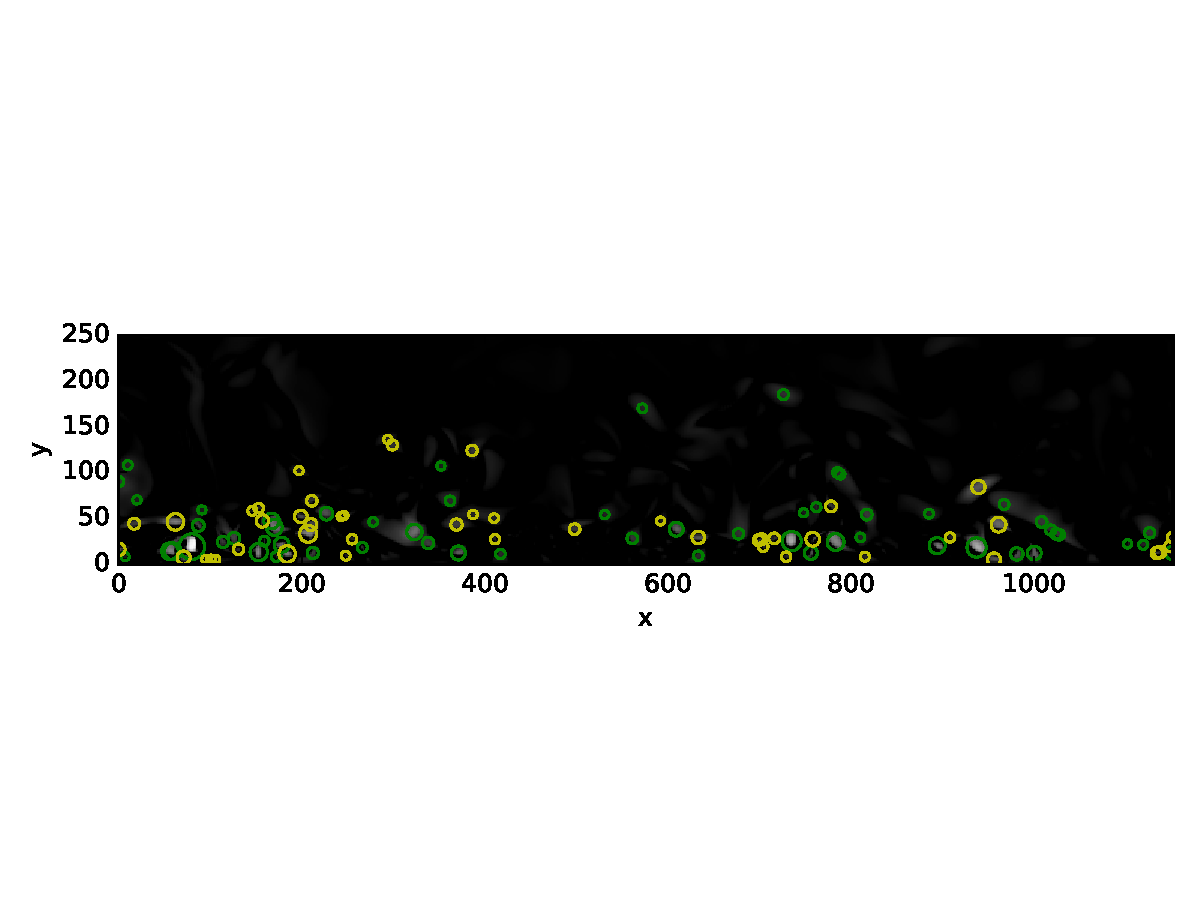
\includegraphics[trim=0 140 0 150 ,clip, width=\textwidth]{figure/PIVnonnormalized.pdf}
	\caption{}
	\label{fig:nonnorm2}
	\end{subfigure}
	\begin{subfigure}[b]{\textwidth}
		\centering
	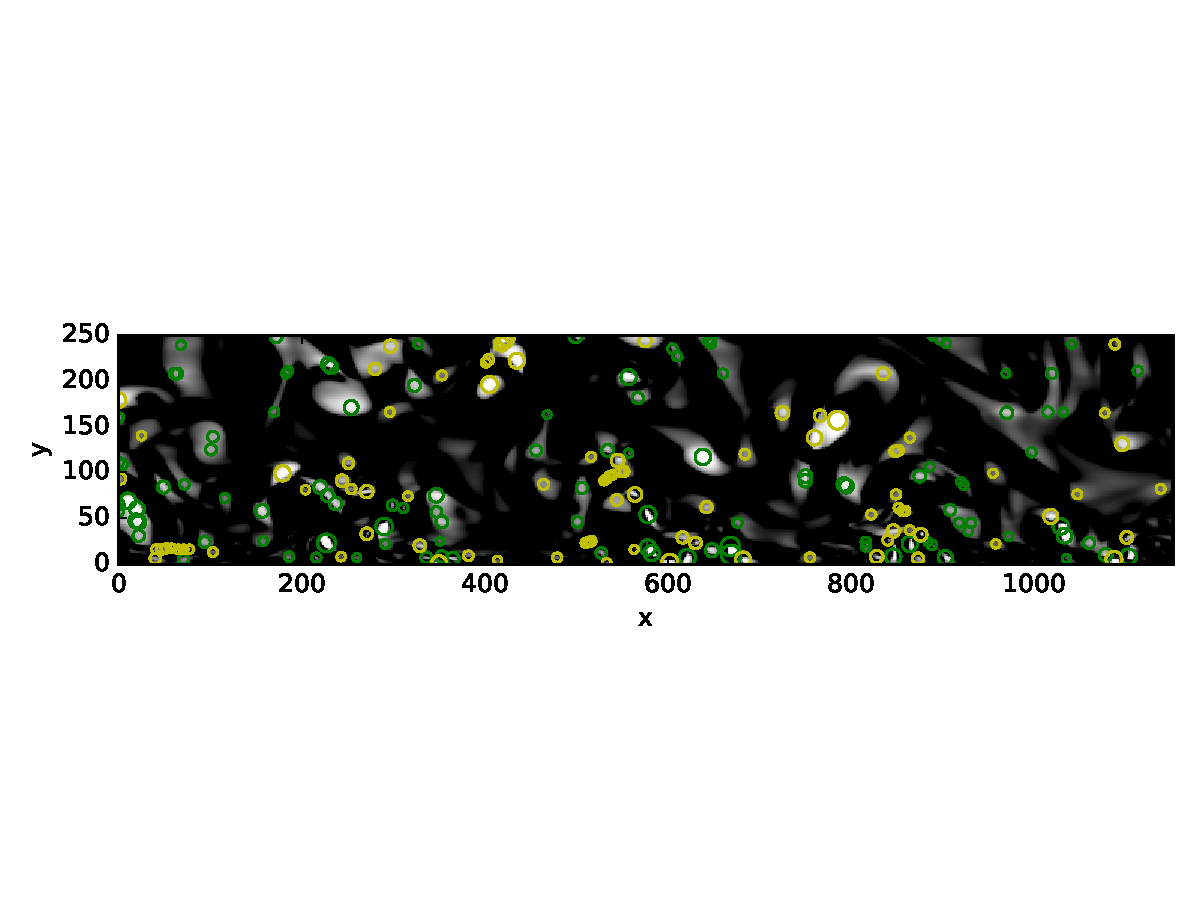
\includegraphics[trim=0 140 0 150 , clip, width=\textwidth]{figure/PIVnormalized.pdf}
	\caption{}
	\label{fig:norm2}
	\end{subfigure}
	\begin{subfigure}[b]{\textwidth}
		\centering
	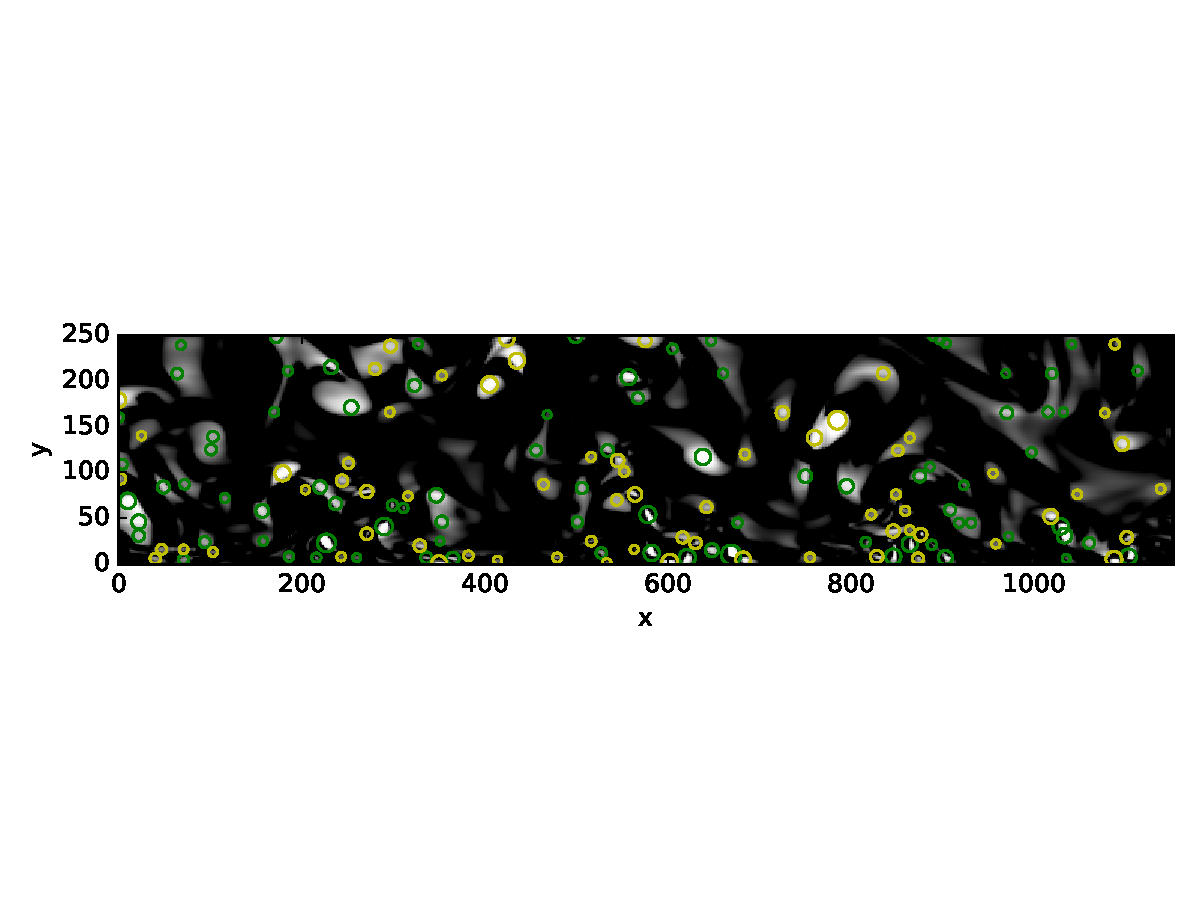
\includegraphics[trim=0 130 0 150 , clip, width=\textwidth]{figure/PIVbox12normalized.pdf}
	\caption{}
	\label{fig:boxnorm2}
	\end{subfigure}
	\caption{PIV swirling strength field, (a) original, (b) fluctuation field, (c) normalized field with boxsize=12 }
	\label{fig:PIVcomparison}
\end{figure}

In figure \ref{fig:nonnorm2} we see the original swirling strength field, where 104 vortices were found, mostly near the wall, where the boundary layer plays an important role in increasing the swirling strengtht. The yellow circles corresponds to the vortices rotating clockwise and the green circles for the counter-clockwise rotation. 

In figure \ref{fig:norm2} we show the fluctuation of the swirling strength field, by applying the Reynolds decomposition, now with 202 vortices found, minimizing the wall influence over the detection.

We can play with the distance between one detected vortex and another, by increasing the box size of the peak detection. In figure \ref{fig:boxnorm2} we set the box size to 12, instead of box size 6 used in figures \ref{fig:nonnorm2} and \ref{fig:norm2}. With this setting we reduce the detected vortices to 154, by removing the overlapping ones.

One interesting fact about the swirling strength (as well the other methods) is that the local maximum values does not always match the center of the vortex. We show in \ref{fig:quiverDNS1} one example of this mismatch between them.

\begin{figure}[h]
	\centering
	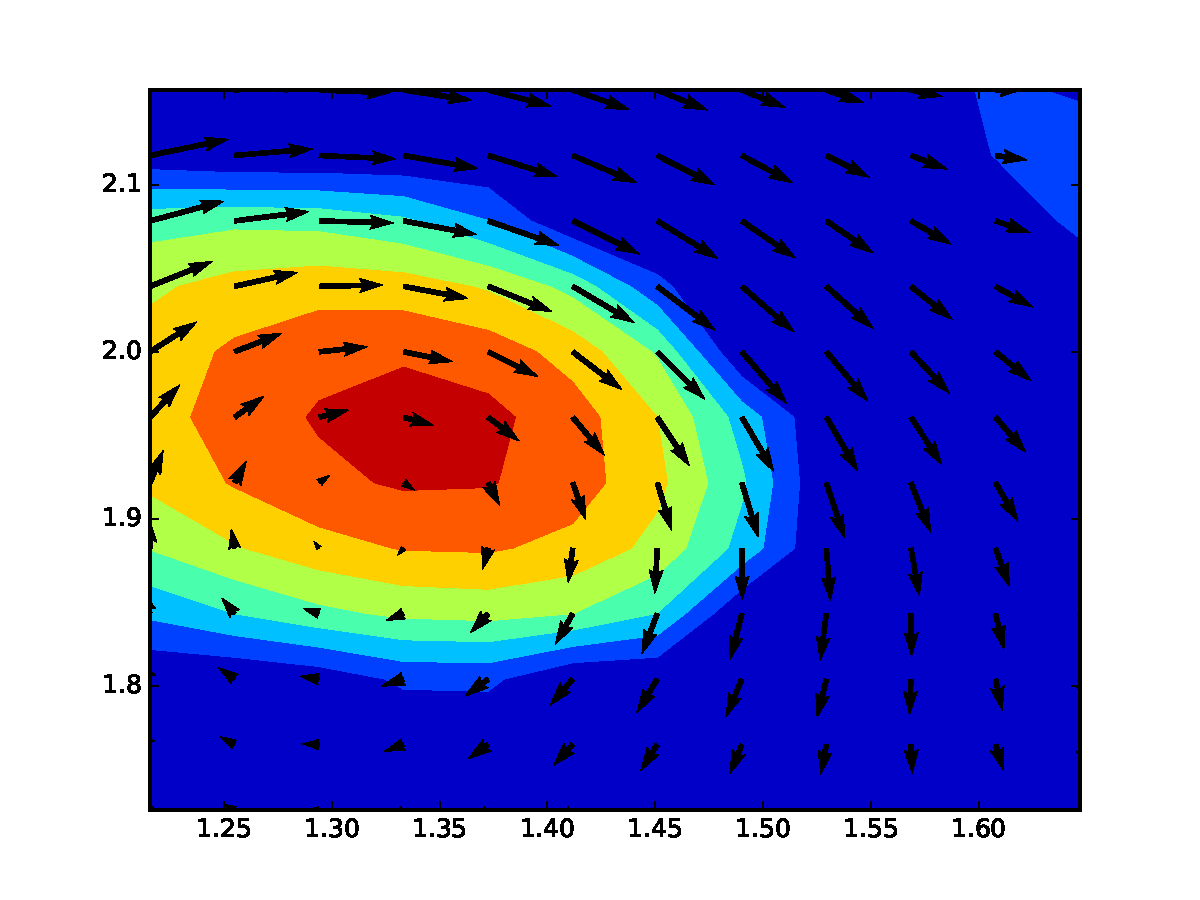
\includegraphics[scale=0.6]{figure/dns_quiver1.pdf}
	\caption{Sample of velocity vectors on top of the swirling strength field}
	\label{fig:quiverDNS1}
\end{figure} 

\section{Fitting of coherent structures}

Using the peak of maximum swirling strength or identifying the places where the Q or $\Delta$ criterion are higher than 0 gives us a rough estimation of a possible vortex and its center. But even using a threshold on these methods, the presence of a real vortex is not always true. To improve this detection we use a Lamb-Oseen vortex model to be fitted on top of the actual detected peak to check if it is really a vortex. 

The correlation coefficient between the fitted model and the velocity field is calculated according to equation \ref{eq:corr} and if it's higher than 0.75 we can consider it a vortex.

\begin{equation}
\label{eq:corr}
R(model/data) = \left( \frac{\langle (\vec{u}_{data}-\vec{u}_c).(\vec{u}_{model}-\vec{u}_c)\rangle }
{\sqrt{\langle (\vec{u}_{data}-\vec{u}_c)^2\rangle} \sqrt{\langle (\vec{u}_{model}-\vec{u}_c)^2\rangle}} \right)^{1/2}
\end{equation}

\subsection{Lamb-Oseen vortex}

The Lamb-Oseen vortex is a mathematical model for the flow velocity in the circumferential direction ($\theta$), shown in equation \ref{eq:oseenDecay}. It models a line vortex that decays due to viscosity.

\begin{equation}
\label{eq:oseenDecay}
\vec{u}_\theta(r,t) = \frac{\Gamma}{2\pi r} \left( 1 - exp \left( -\left(\frac{r}{r_0(t)}\right)^2\right)\right) \vec{e}_{\theta}
\end{equation}
where $r$ is the radius, $r_0 = \sqrt{4 \nu t}$ is the core radius of vortex, $\nu$ is the viscosity and $\Gamma$ is the circulation contained in the vortex. 

In this work we are dealing with a time-independent flow, so we have no decaying due to viscosity. And since the coherent structures are in movement, we add the convective velocity to the Lamb-Oseen vortex model shown in equation \ref{eq:oseen}.  

\begin{equation}
\label{eq:oseen}
\vec{u}(r,\theta) = \vec{u}_c + \frac{\Gamma}{2\pi r} \left( 1 - exp \left( -\left(\frac{r}{r_0}\right)^2\right)\right) \vec{e}_{\theta}
\end{equation}

\subsection{Non-linear least squares}

\subsubsection{Levenberg Marquardt method}

The Levenberg–Marquardt algorithm, also known as the damped least-squares method, is used to solve non-linear least squares problems. These minimization problems arise especially in least squares curve fitting.

\begin{equation}
\chi^2 = \sum_{i=1}^N \left[ \frac{y_i - \sum_{k=1}^M a_k X_k (x_i)}{\sigma i} \right]^2
\end{equation}

\begin{equation}
\alpha_{kl} = \sum_{i=1}^N \frac{1}{\sigma_i^2} \left[ \frac{\partial y(x_i;a)}{\partial a_k} \frac{\partial y(x_i;a)}{\partial a_l} \right]
\end{equation}

\subsubsection{Powell's dogleg method}

The Powell's method is an algorithm for finding a local minimum of a function. This function doesn't need to be differentiable and no derivatives are taken. It does this using a combination of Newton's method and the steepest descent method. This is a so-called trust region method. This means that every step moves the current point to within a finite region. This makes the method more stable than Newton's method.

\section{Programming}

The language chosen for developing the detection tools is Python 3.6 (Python Software Foundation, https://www.python.org/). This choice was made for the following reasons:
\begin{itemize}
	\item \textbf{Readability} \\
	Python's syntax is easy to read, very close to pseudocode itself.
	\item \textbf{Access to low level programming languages} \\
	We can easily add C or Fortran code o be run inside Python's code, reusing some useful libraries and tools.
	\item \textbf{Language interoperability} \\
	MATLAB functions can be called from Python through the MATLAB engine and even other languages.
	\item \textbf{Documentation system} \\
	One helpful feature for scientific programming is the ability to put LaTeX equations and plots directly in code documentation, by using the docstrings.
	\item \textbf{Available libraries} \\
	Python has an impressive standard library packaged with Python. For scientific uses, the most well known are NumPy and SciPy.
\end{itemize} 

\newpage
\subsection{Code Structure}

The following files are present on the code, allowing the easy implementation of new methods, tools or scheemes.

\begin{itemize}
	\item vortexfitting.py : main program
	\item classes.py : definition of the data type, i.e. DNS, PIV, ...
	\item detection.py : detect the vortices by one of the methos (Q criterion, $\lambda_2$ criterion or swirling strenth)
	\item fitting.py : performs the fit to oseen vortex
	\item plot.py : plot the desired results, like scalar fiels, vectors, ...
	\item schemes.py : differencing schemes (2nd and 4th order)
	\item testoseen.py : tests for fitting performance
	\item tools.py : normalization, vortex window definition, local maxima detection, ... 
\end{itemize}

The code uses the version control system Git, and it's hosted and fully available at \url{https://github.com/guilindner/VortexFitting}. 

\newpage
\subsection{Routine}

Here we describe in the figure \ref{fig:mainprogramfc} the routine done by the main program, as well the details of the fitting routine on figure \ref{fig:fittingfc}. Currently the user must specify on the \textit{classes.py} file if the data have one homogeneous direction or not, so the proper normalization and smoothing can be done by the routine if required.

\begin{figure}[h!]
	\centering
	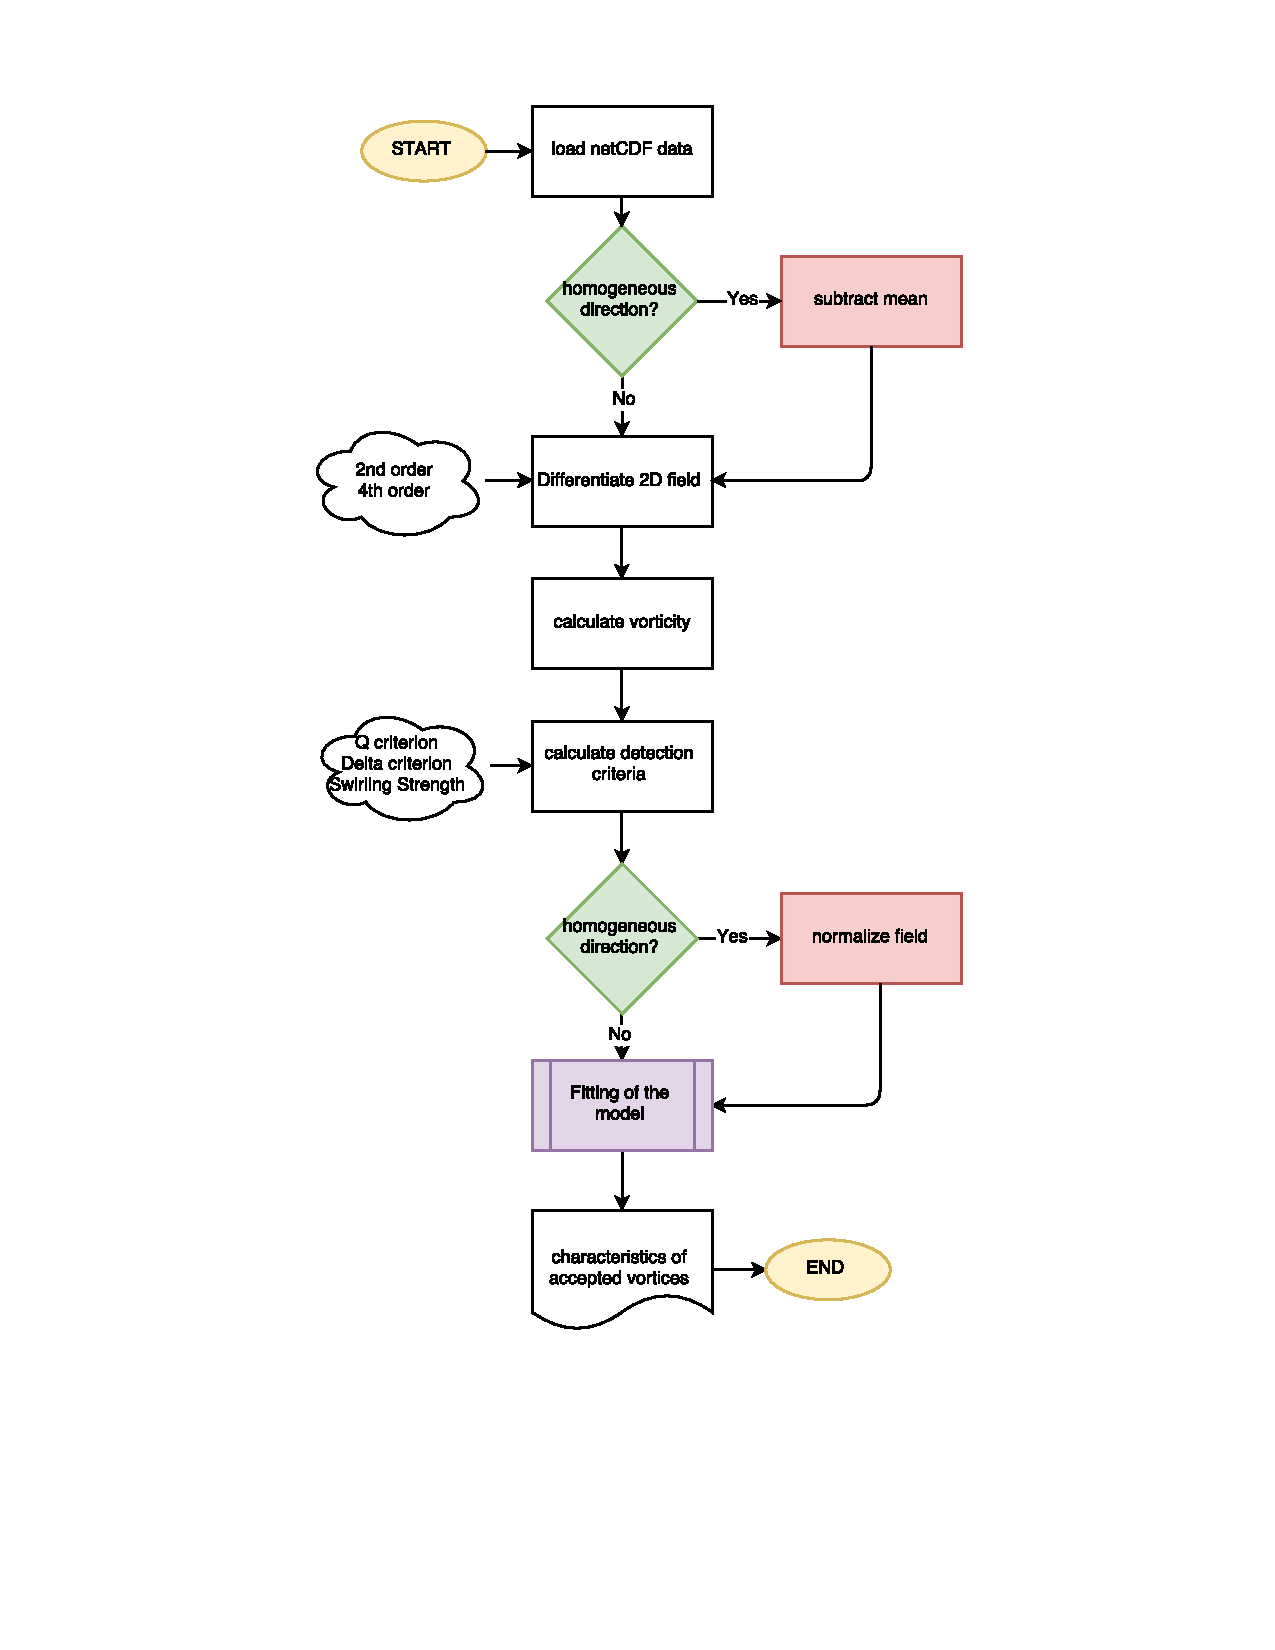
\includegraphics[trim=150 150 150 50 ,clip, scale=0.8]{figure/vortexFittingFlow.pdf}
	\caption{flowchart of the main program.}
	\label{fig:mainprogramfc}
\end{figure}

\newpage
\begin{figure}[h!]
	\centering
	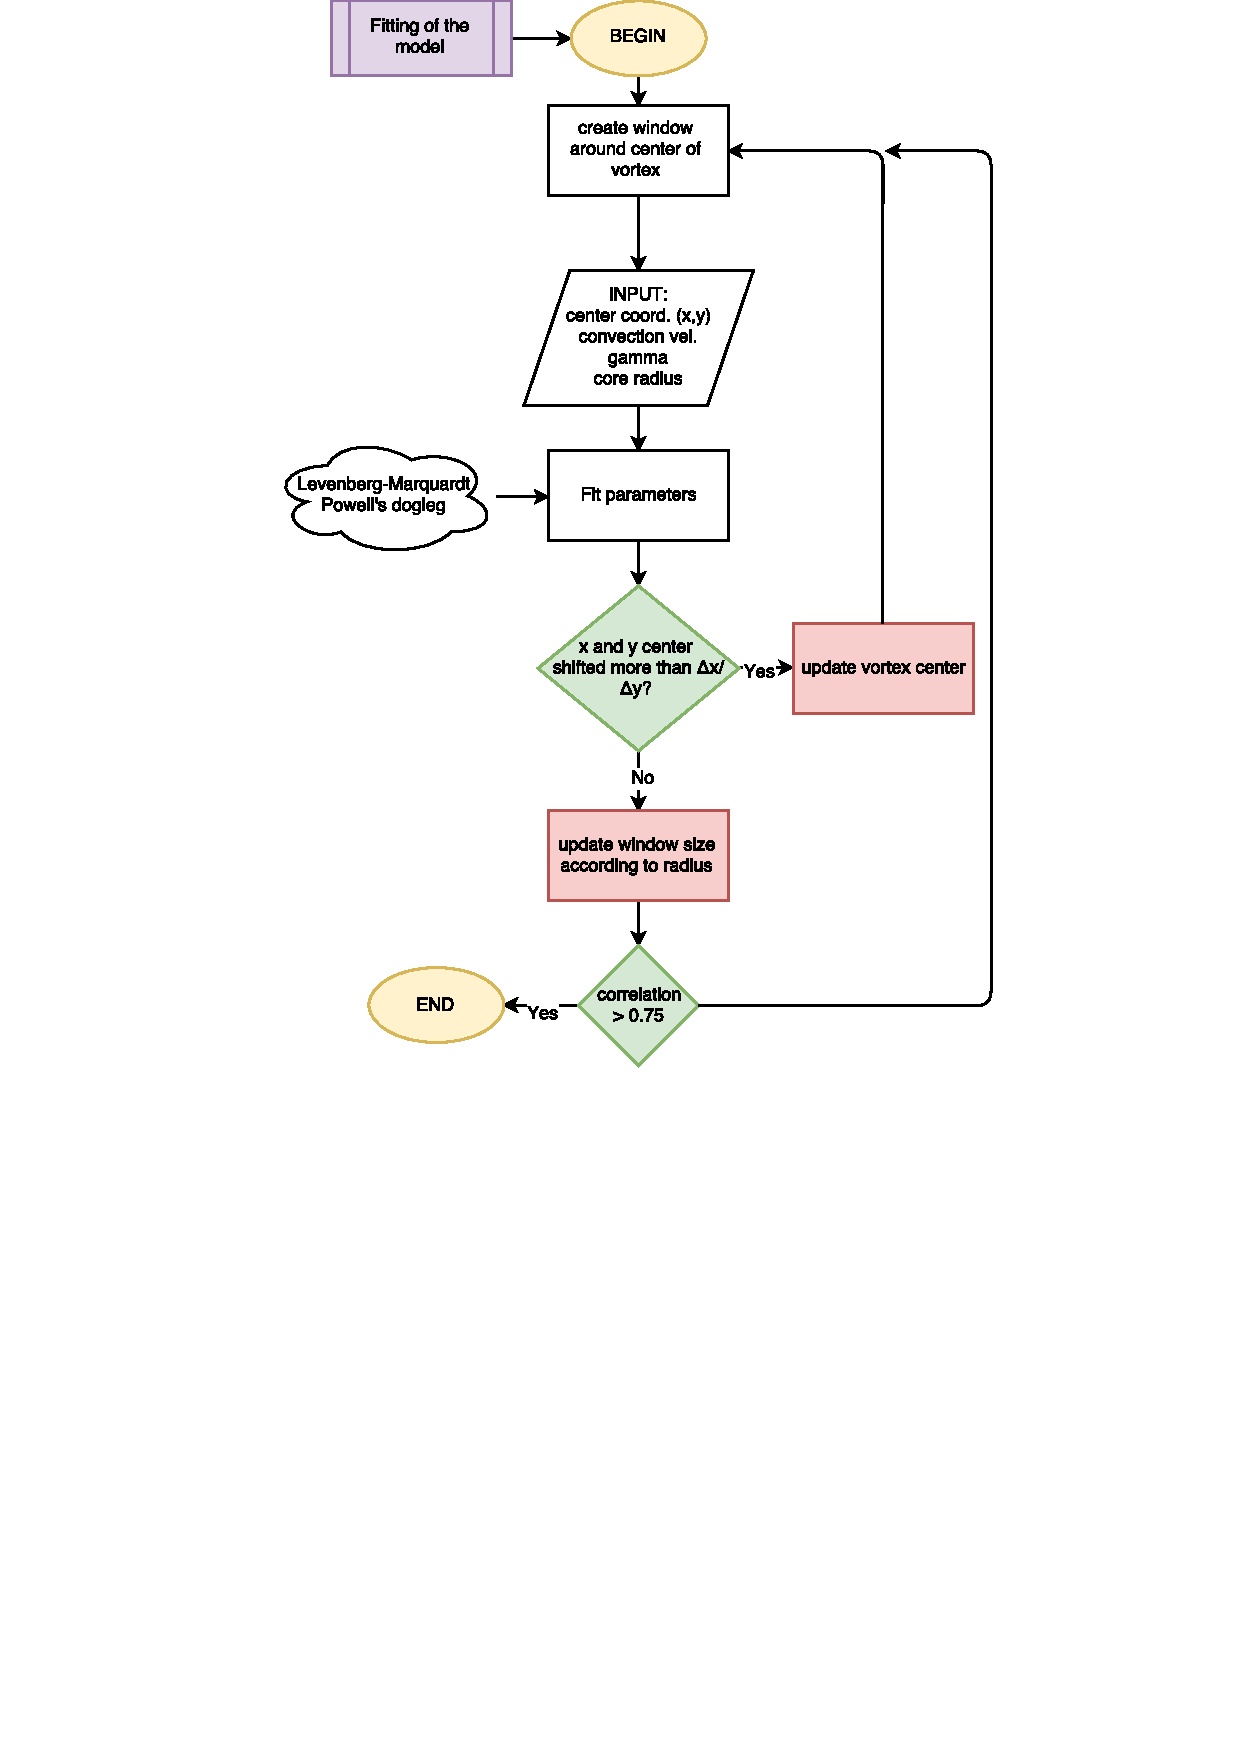
\includegraphics[trim=50 320 50 0 ,clip, scale=0.8]{figure/FittingFlow.pdf}
	\caption{Detailed flowchart of the "Fitting of the model".}
	\label{fig:fittingfc}
\end{figure}

This iteration loop allows the fitting window to be adjusted according to the core radius of the vortex, and simultaneously change the center position of the vortex if needed. 

\chapter{Validation}
In this chapter we will use some controlled cases to test the overall performance of the code.

\section{Detection}
Here we will test the three detection methods, Q criterion, $\Delta$ criterion and swirling strength.

For the derivative scheme, we will use the 4th order accurate scheme and 2nd order (details on Annnex \ref{annex:finite}). According to Raffel \textit{et al} (1998), the 2nd order scheme is recommended because it minimizes the propagation of measurement noise.   

The tested case is an Homogeneous Isotropic Turbulence (HIT) of a cube, obtained from Direct Numerical Simulation (DNS) calculations.

\begin{table}[h]
	\centering
	\caption{Vortices found, detection X schemes}
	\vspace{10px}
	\label{tb:detection}
	\begin{tabular}{l|c|c}
		         & 2nd order      & 4th order  \\
		\hline
		Q criterion  & 403  & 398  \\
		$\Delta$ criterion & 462  & 462 \\
		Swirling strength    & 413  & 409
	\end{tabular}
\end{table}

\section{Fitting}

In this section we will test the Oseen Vortex model fitting under different scenarios. For the first comparison a standard Oseen Vortex is created to be an exact match and for the second set of tests we add a noise to the original vortex field.

Figures \ref{fig:fittingtests} and \ref{fig:fittingtestsnoise} shows 4 different cases, varying the core radius, $\Gamma$ and the distance of the center of vortex to the center of window (shift).

\begin{figure}[h!]
	\centering
	\begin{subfigure}[b]{0.45\textwidth}
		\centering
		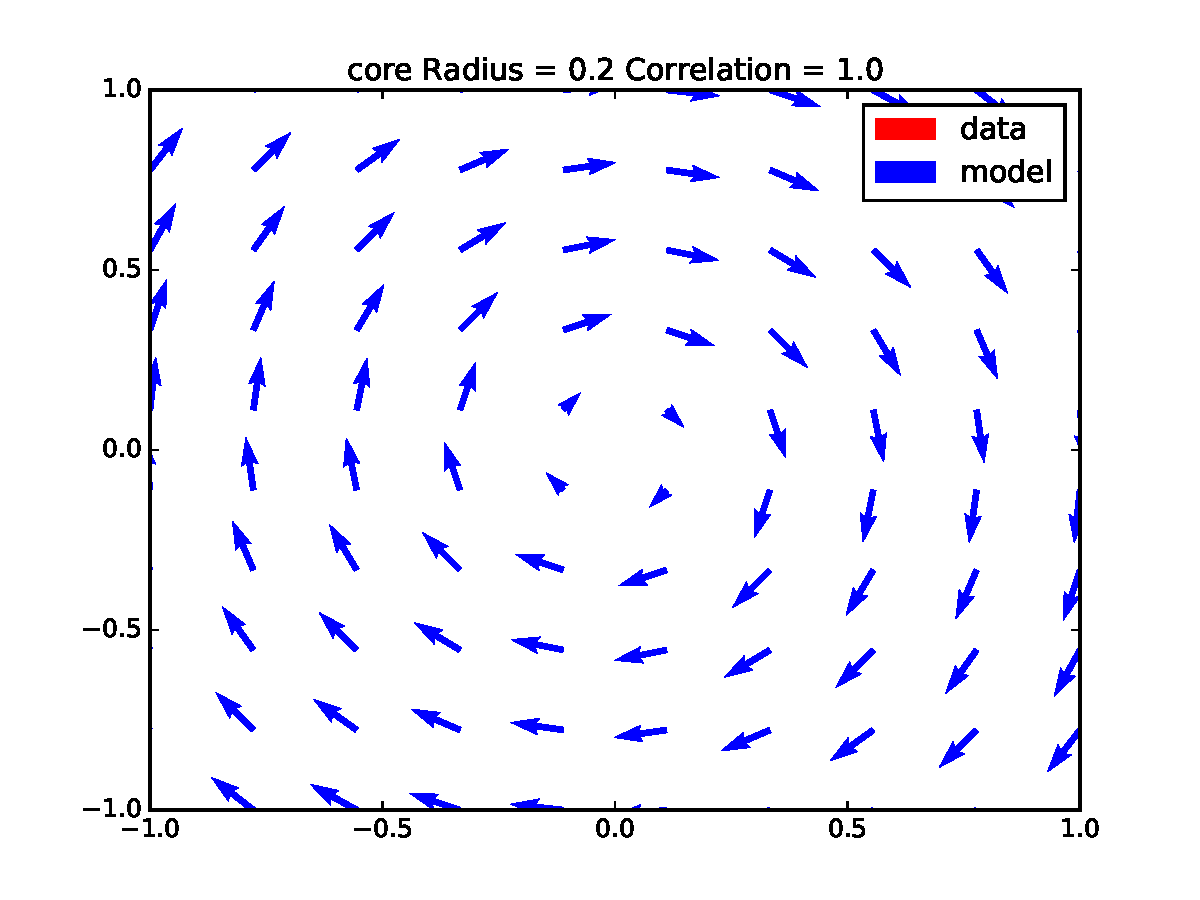
\includegraphics[trim=40 20 40 20 ,clip, width=\textwidth]{figure/test_02_10.pdf}
		\caption{Initial values: r = 0.2, $\Gamma$ = 10}
	\end{subfigure}
	\begin{subfigure}[b]{0.45\textwidth}
		\centering
		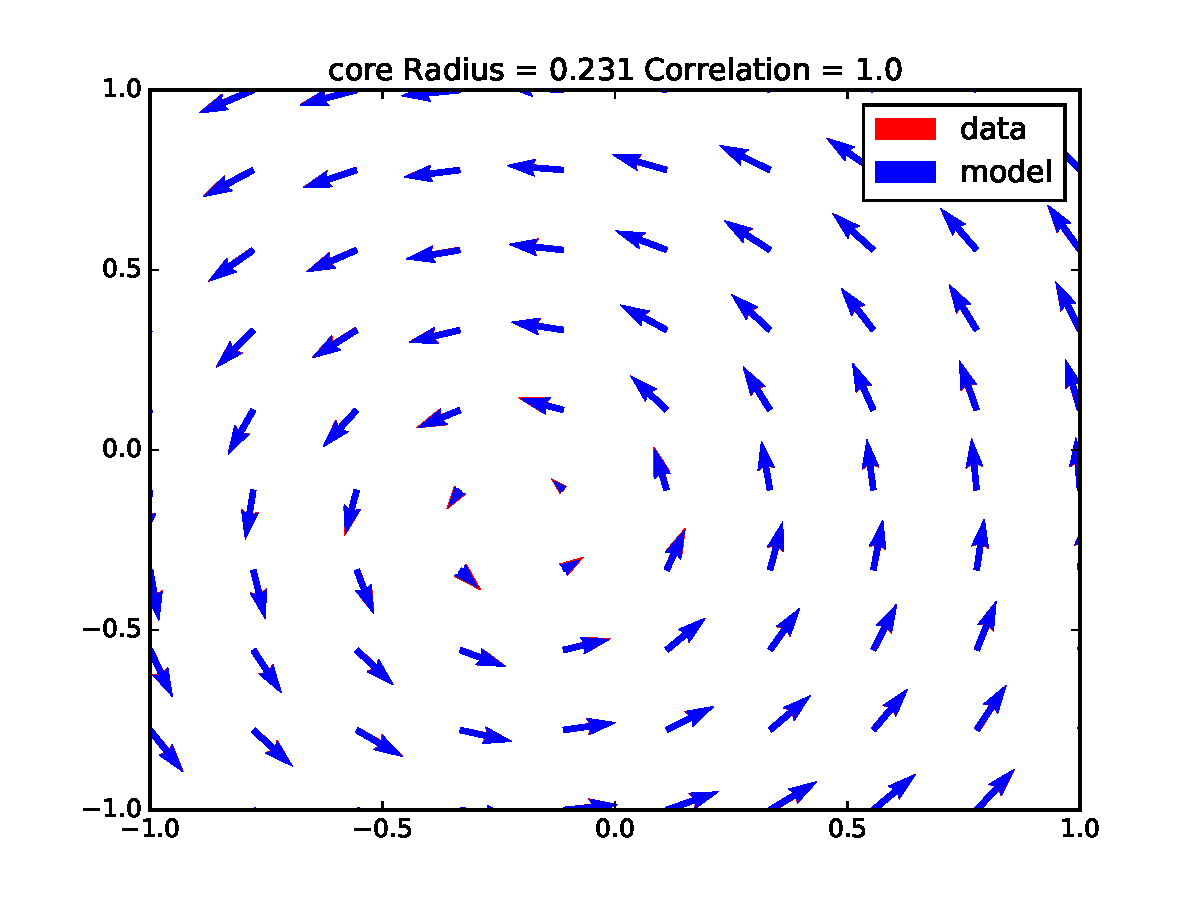
\includegraphics[trim=40 20 40 20 ,clip, width=\textwidth]{figure/test_02_10_02.pdf}
		\caption{r = 0.2, $\Gamma$ = 10, shift = 0.2}
	\end{subfigure}
	\begin{subfigure}[b]{0.45\textwidth}
		\centering
		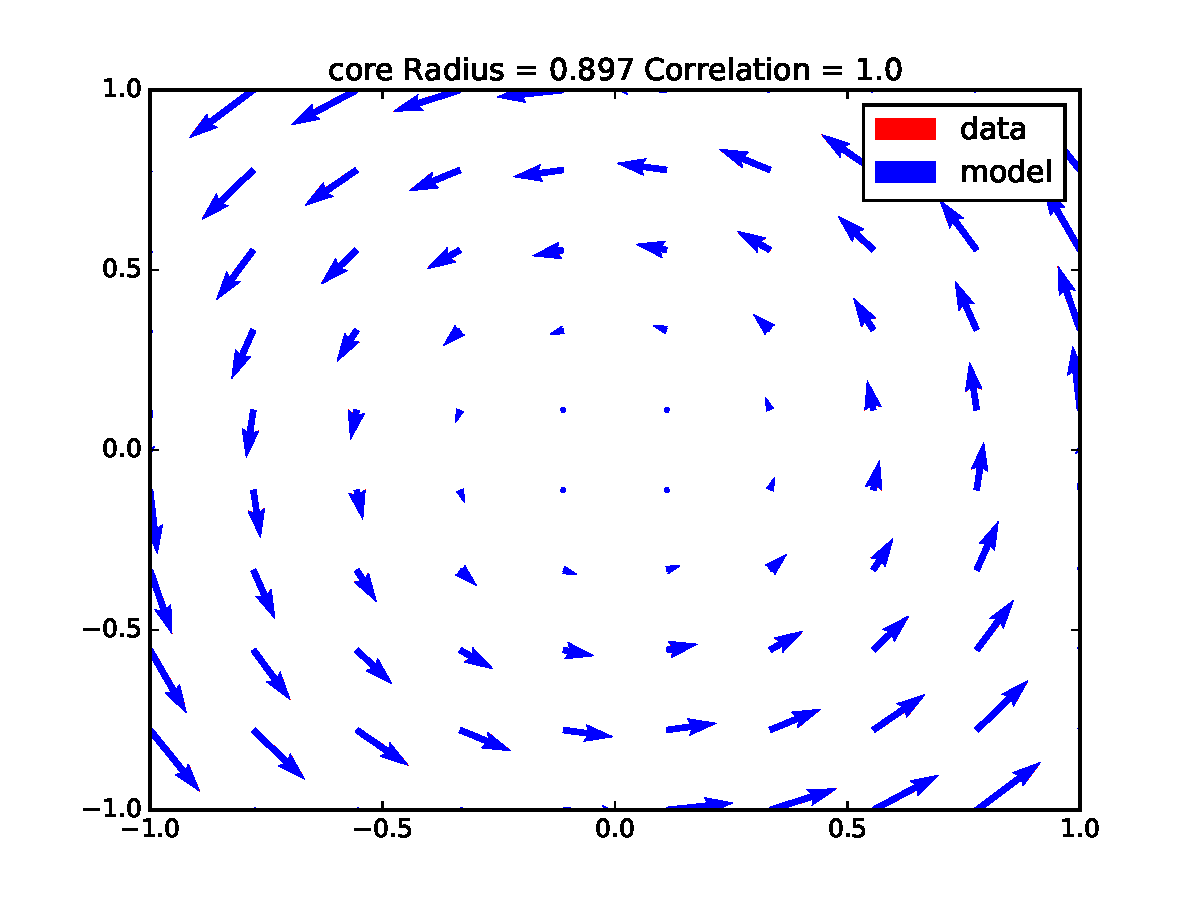
\includegraphics[trim=40 20 40 20 ,clip, width=\textwidth]{figure/test_09_40.pdf}
		\caption{Initial values: r = 0.9, $\Gamma$ = 40}
	\end{subfigure}
	\begin{subfigure}[b]{0.45\textwidth}
		\centering
		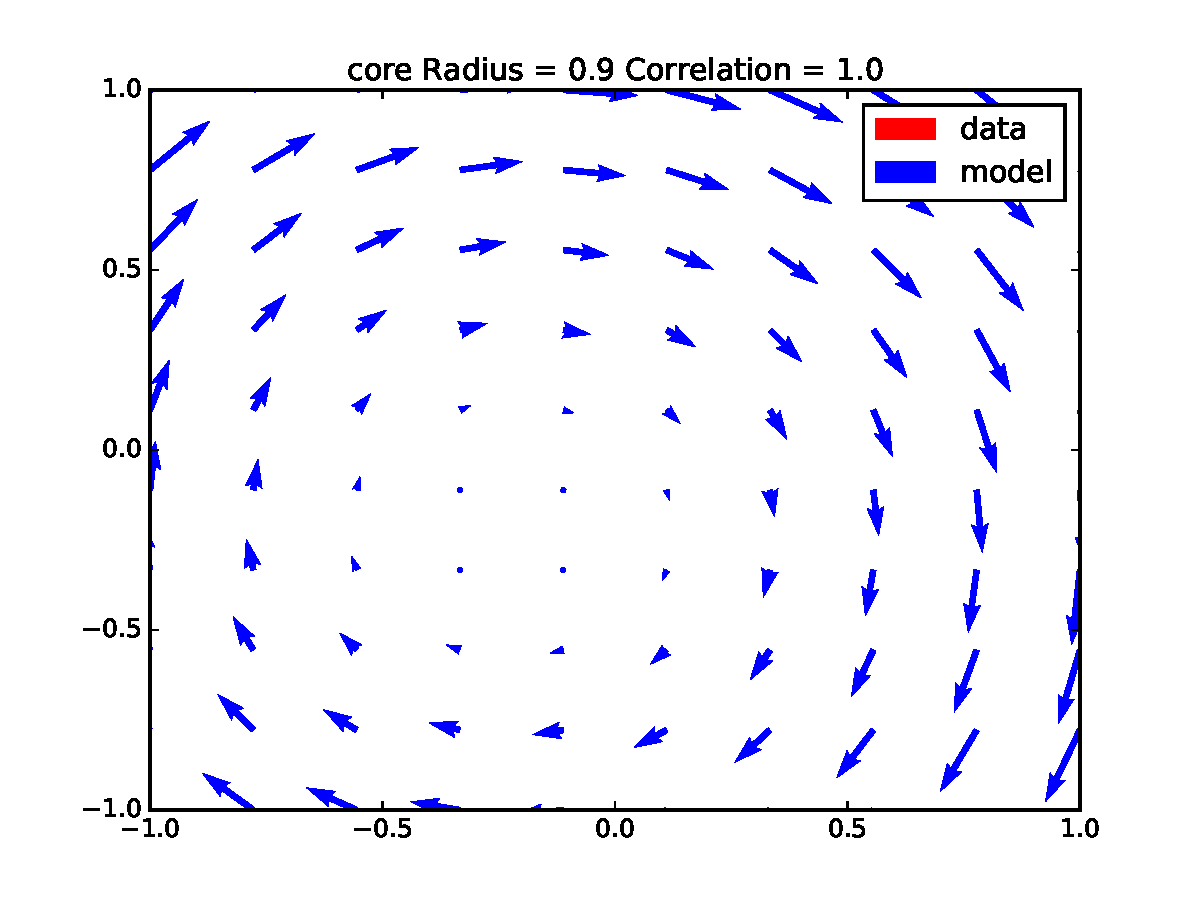
\includegraphics[trim=40 20 40 20 ,clip, width=\textwidth]{figure/test_09_40_02.pdf}
		\caption{r = 0.9, $\Gamma$ = 40, shift = 0.2}
	\end{subfigure}
	\caption{Fitting test}
	\label{fig:fittingtests}
\end{figure}

\begin{table}[h]
	\centering
	\caption{Velocity vectors of the fitting test}
	\vspace{10px}
	\label{tb:fittingtest}
	\begin{tabular}{l|c|c|c|c}
		            & a      & b & c & d \\
		\hline
		radius      & 0.2000   & 0.2000 & 0.9000 & 0.8999  \\
		$\Gamma$       & 10.0000 & 10.0000 & 40.0000 & 39.9999 \\
		x shift     & 0.0000  & 0.2000 & 0.0000 & 0.2000 \\
		y shift     & 0.0000  & 0.2000 & 0.0000 & 0.2000 \\ 
		correlation & 1.0000   & 1.0000 & 1.0000 & 1.0000 \\
	\end{tabular}
\end{table}

We can see in table \ref{tb:fittingtest} that the guess is exact for all the cases, as the vectors totally overlaps themselves (figure \ref{fig:fittingtests}).

Now we add a perturbation to the initial flow field. Considering a random noise of magnitude 0.3 on the on the velocity field, we have the following performance of the fitting presented on table \ref{tb:fittingtestnoise} in respect to the figures \ref{fig:fittingtestsnoise}. The magnitude of the noise is the same on all cases, and since cases c and d have bigger radius and $\Gamma$ (stronger vortices), they are less affected by the noise.

\begin{figure}[h!]
	\centering
	\begin{subfigure}[b]{0.45\textwidth}
		\centering
		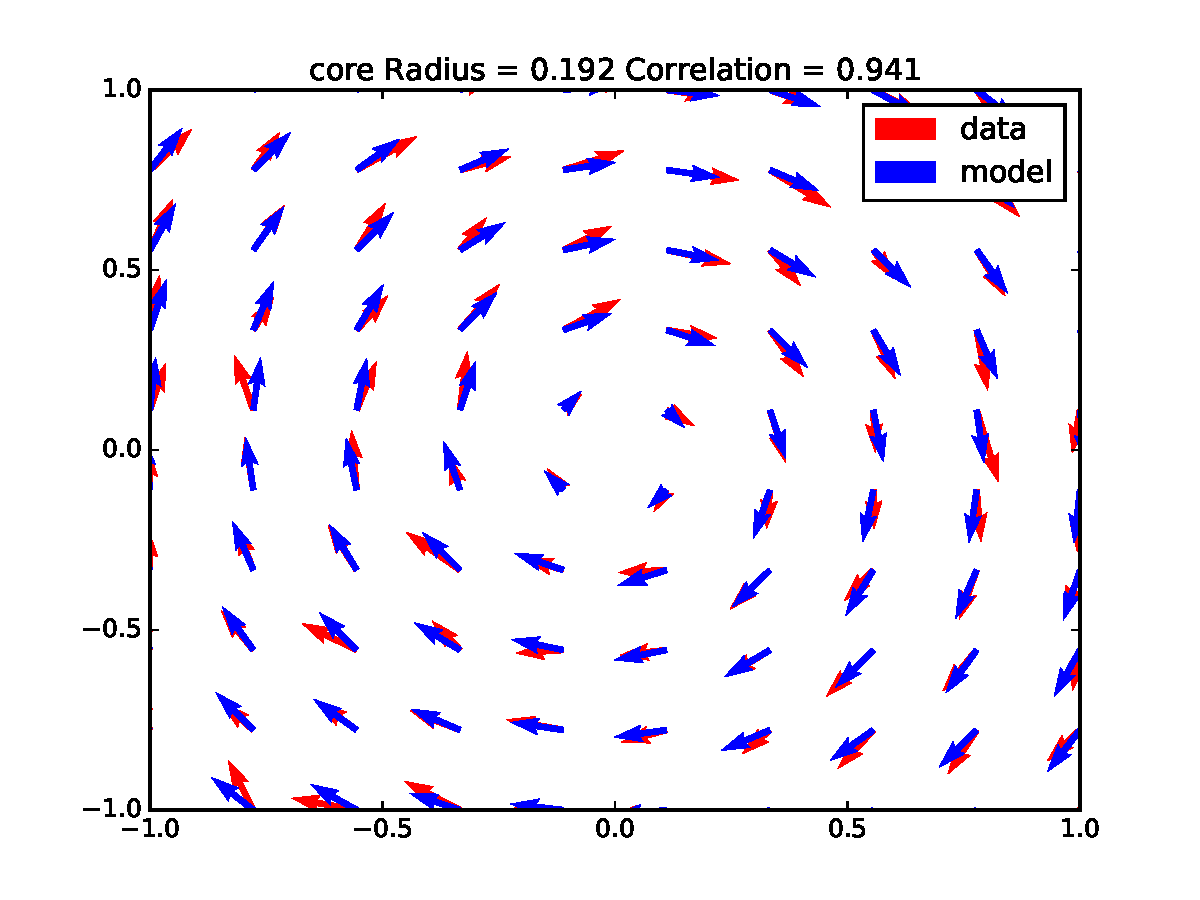
\includegraphics[trim=40 20 40 20 ,clip, width=\textwidth]{figure/test_02_10N.pdf}
		\caption{Initial values: r = 0.2, $\Gamma$ = 10}
	\end{subfigure}
	\begin{subfigure}[b]{0.45\textwidth}
		\centering
		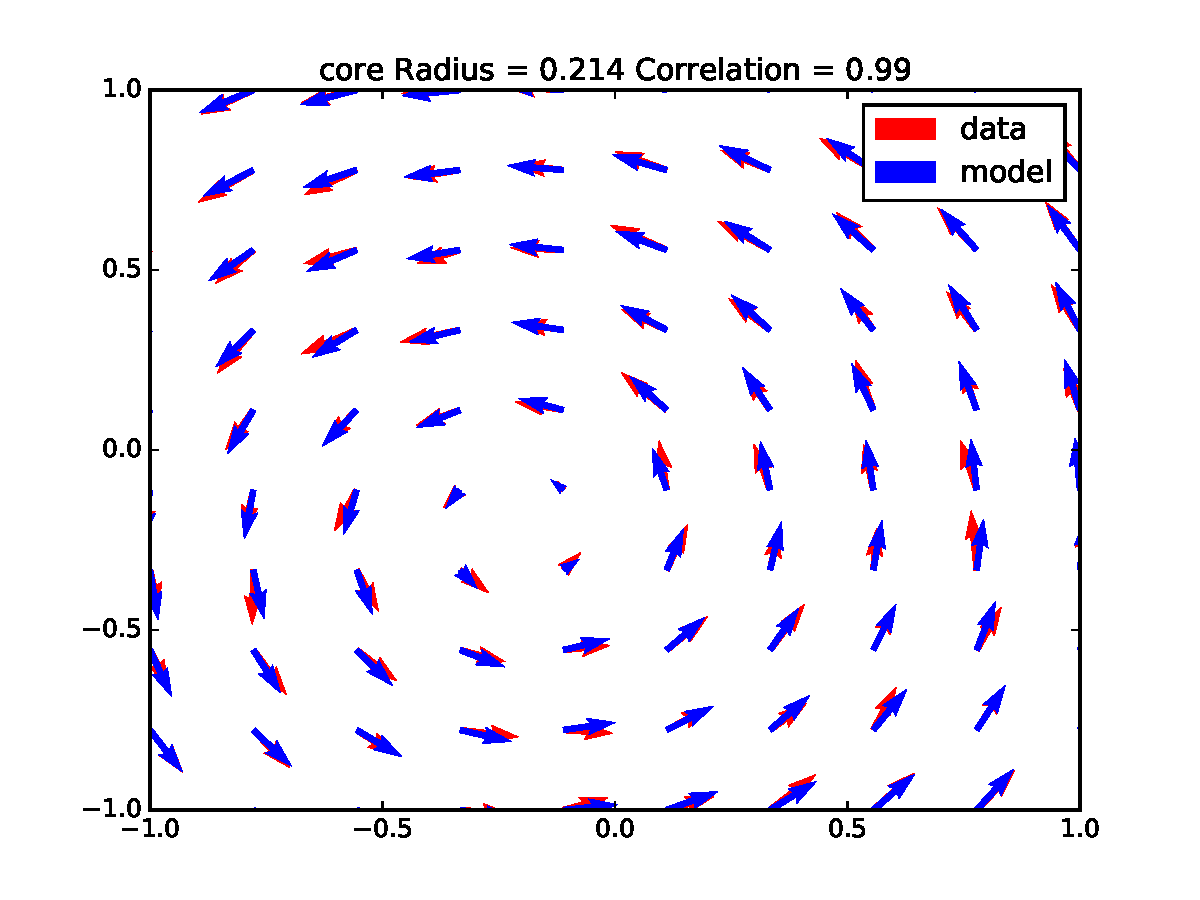
\includegraphics[trim=40 20 40 20 ,clip, width=\textwidth]{figure/test_02_10_02N.pdf}
		\caption{r = 0.2, $\Gamma$ = 10, shift = 0.2}
	\end{subfigure}
	\begin{subfigure}[b]{0.45\textwidth}
		\centering
		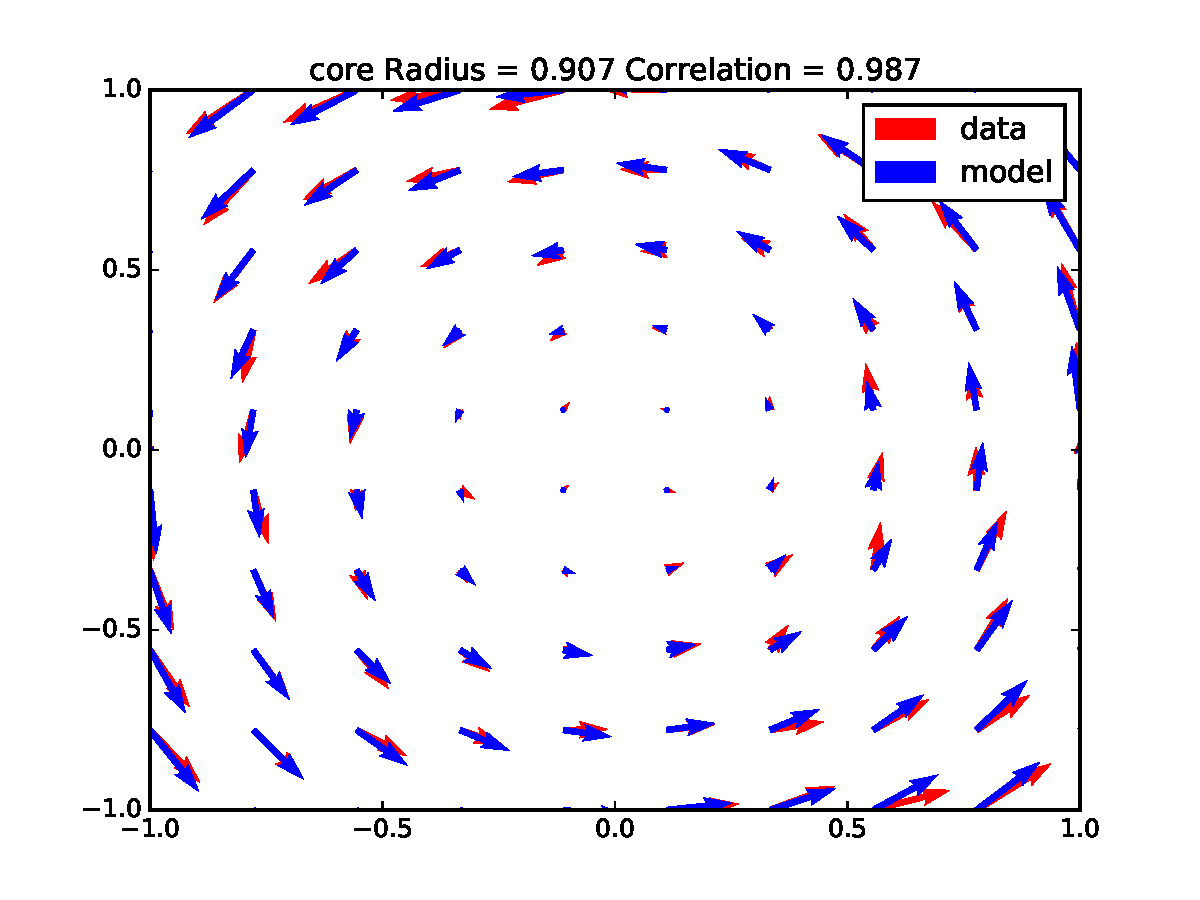
\includegraphics[trim=40 20 40 20 ,clip, width=\textwidth]{figure/test_09_40N.pdf}
		\caption{Initial values: r = 0.9, $\Gamma$ = 40}
	\end{subfigure}
	\begin{subfigure}[b]{0.45\textwidth}
		\centering
		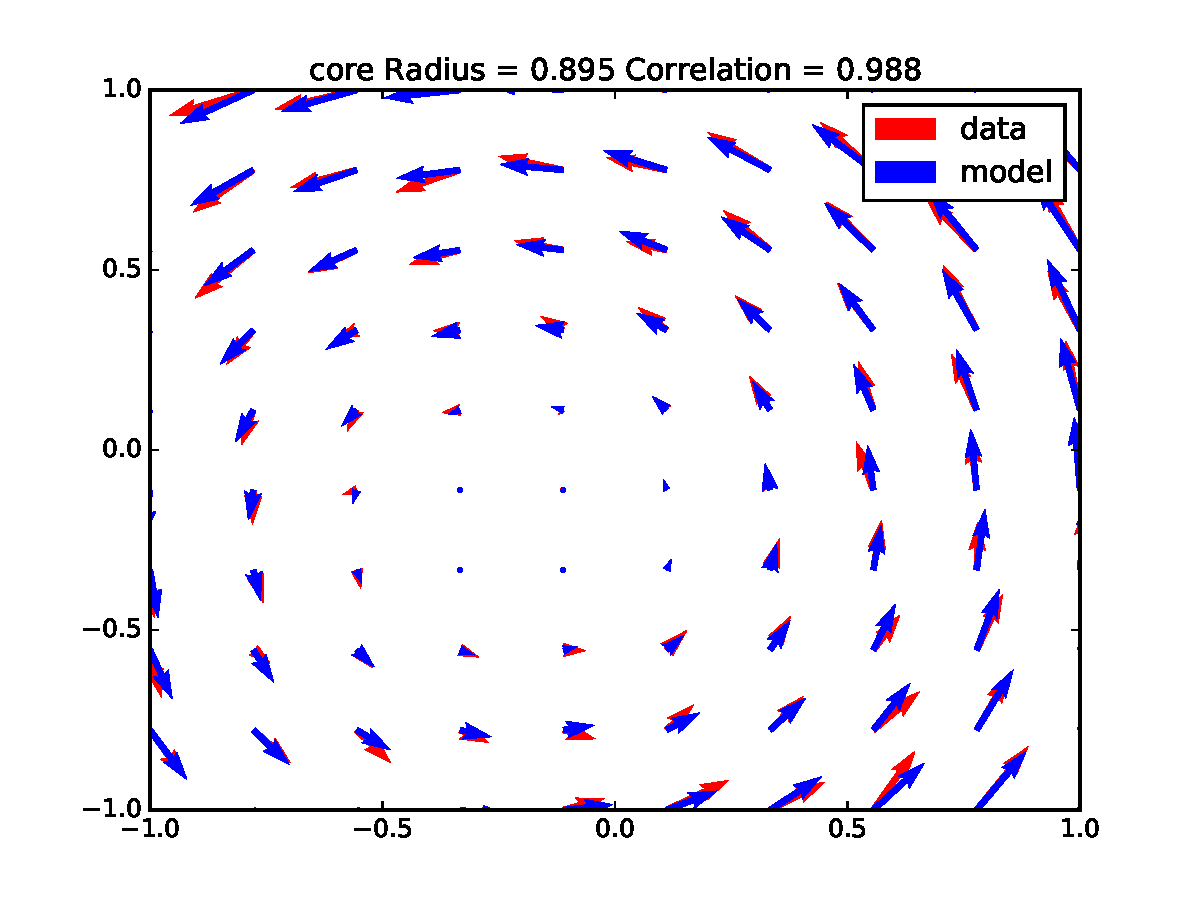
\includegraphics[trim=40 20 40 20 ,clip, width=\textwidth]{figure/test_09_40_02N.pdf}
		\caption{r = 0.9, $\Gamma$ = 40, shift = 0.2}
	\end{subfigure}
	\caption{Velocity vectors of the fitting test with random noise added}
	\label{fig:fittingtestsnoise}
\end{figure}

\begin{table}[h]
	\centering
	\caption{Fitting test results with noise}
	\vspace{10px}
	\label{tb:fittingtestnoise}
	\begin{tabular}{l|c|c|c|c}
		            & a      & b & c & d \\
		\hline
		radius      & 0.1917   & 0.2427 & 0.9067 & 0.9169  \\
		$\Gamma$       & 10.1863 & 9.9743 & 40.4885 & 40.5987 \\
		x shift     & 0.0035  & 0.1946 & -0.0098 & 0.1953 \\
		y shift     & 0.0028  & 0.1918 & 0.0085 & 0.1995 \\ 
		correlation & 0.9406   & 0.9153 & 0.9895 & 0.9869 \\
	\end{tabular}
\end{table}


\chapter{Results}
Here we show the results of the full fitting procedure of DNS data.

\section{DNS data}
This case is an homogeneous isotropic turbulence (HIT) study, generated by a DNS simulation. Since we have no walls and boundaries, no normalization of the velocity field or smoothing on the swirling field is needed. The scheme used is the second order central scheme and using the swirling strength criteria for detection.

The swirling strength field, along with the velocity vectors, is shown in figure \ref{fig:swirling}. Only the big recirculation areas can be seen due to the density of vectors.

\begin{figure}[h]
	\centering
	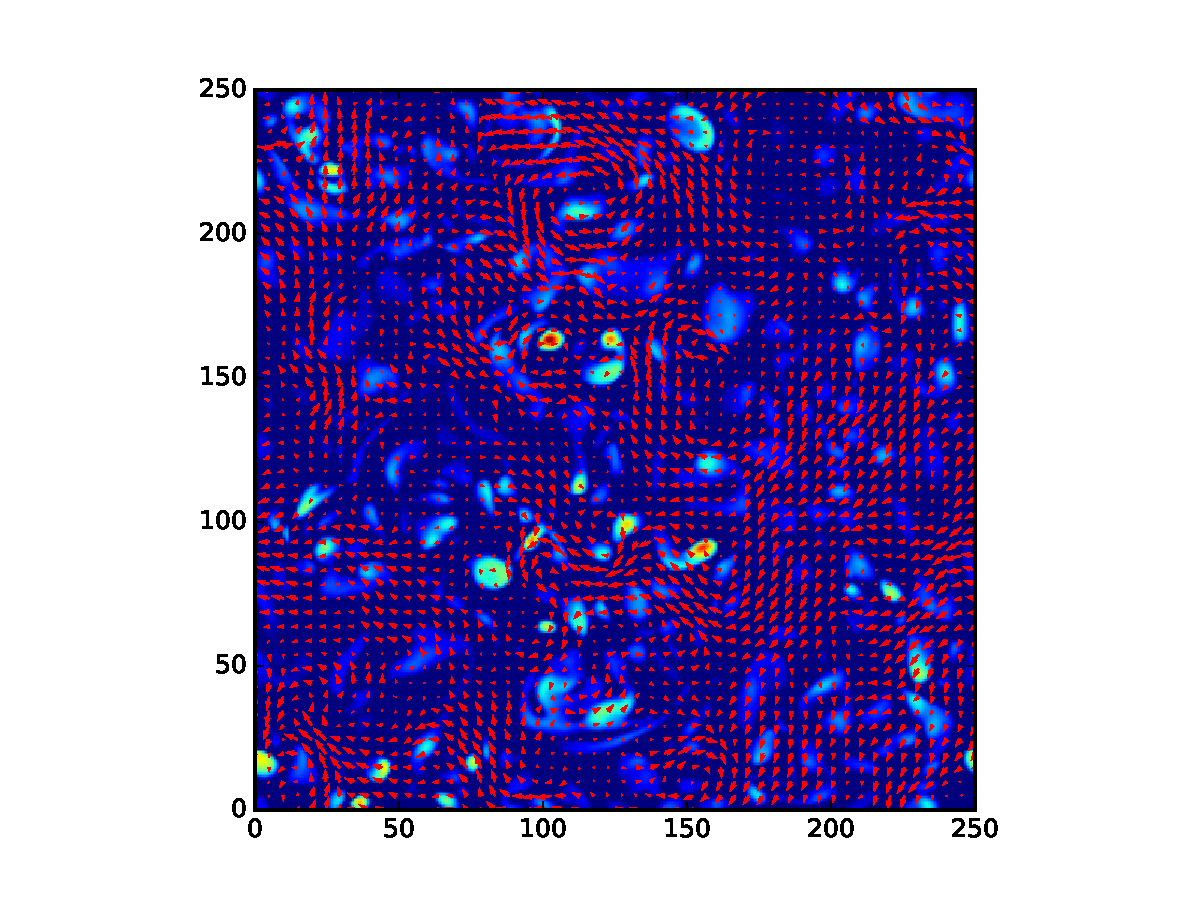
\includegraphics[scale=0.6]{figure/swirling_vector.pdf}
	\caption{Swirling strength field from the DNS with velocity vectors.}
	\label{fig:swirling}
\end{figure}

\begin{figure}[h]
	\centering
	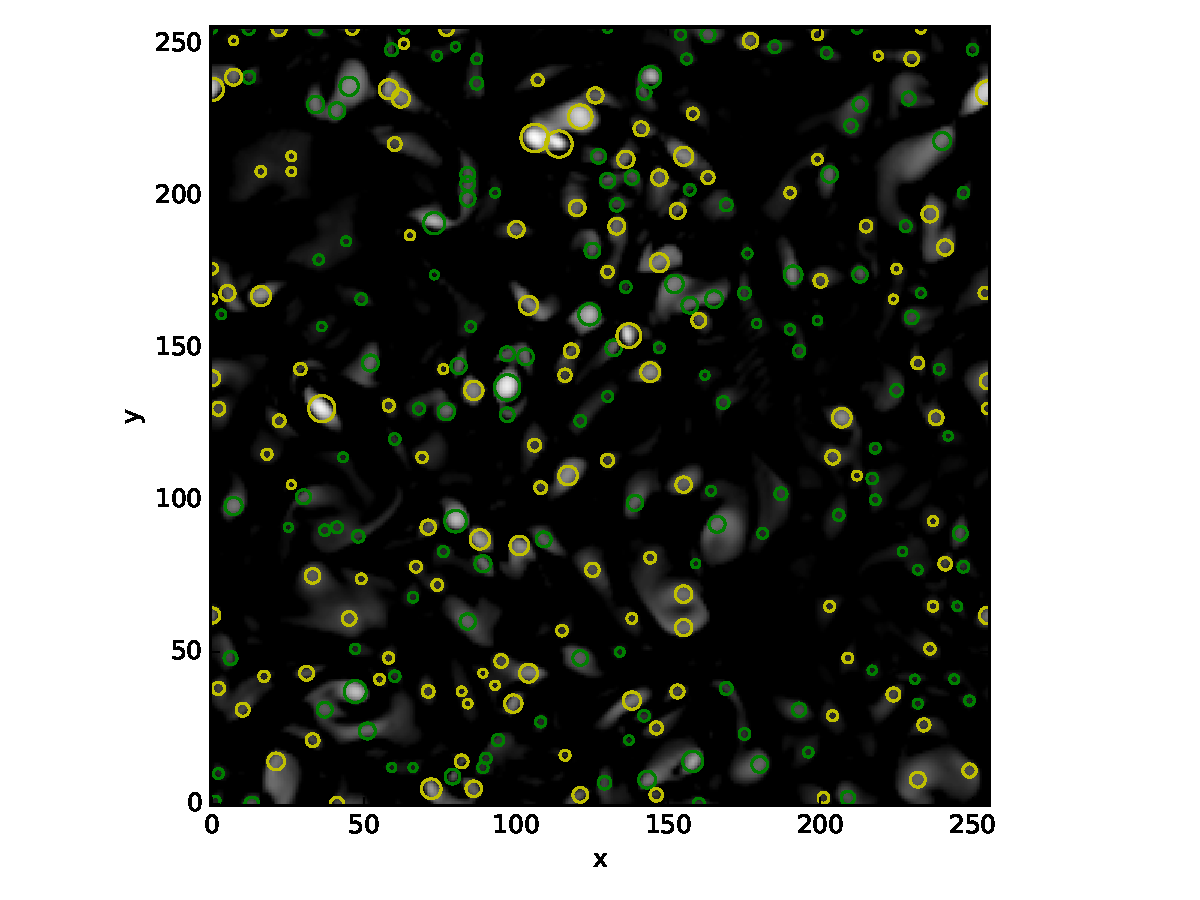
\includegraphics[scale=0.6]{figure/dns_detect.pdf}
	\caption{Detected vortices from the DNS data.}
	\label{fig:detectionDNS}
\end{figure}

After applying the local maxima detection, we see that in figure \ref{fig:detectionDNS}, 278 peaks of swirling strength (vortices candidates) were found, where the yellow circles corresponds to the detected vortices rotating clockwise and the green circles for the counter-clockwise rotation. From these vortices, only 23 were accepted as having a correlation higher than 0.75 with the lamb-oseen vortex.

\begin{figure}[h!]
	\centering
	\begin{subfigure}[b]{0.45\textwidth}
		\centering
		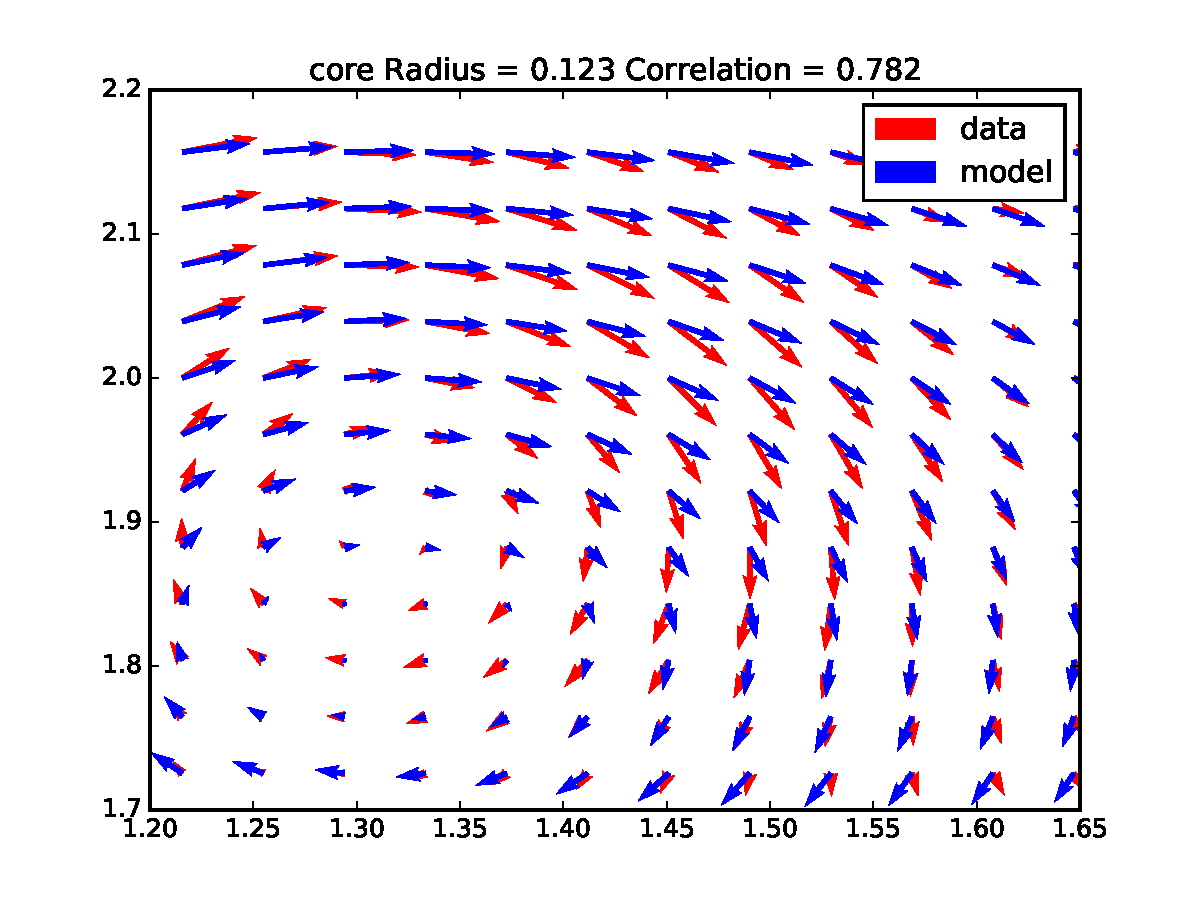
\includegraphics[trim=40 20 40 20 ,clip, width=\textwidth]{figure/dns_fit1.pdf}
		\caption{}
	\end{subfigure}
	\begin{subfigure}[b]{0.45\textwidth}
		\centering
		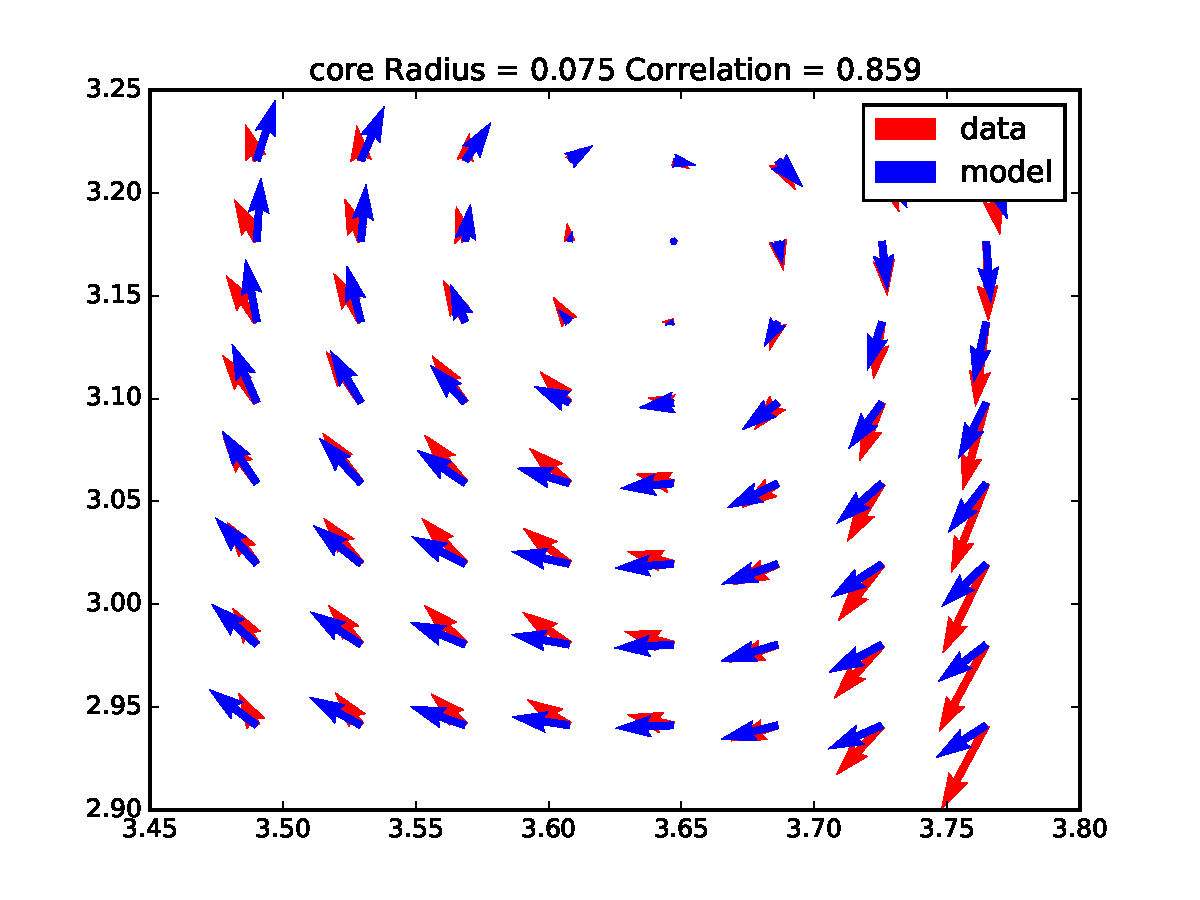
\includegraphics[trim=40 20 40 20 ,clip, width=\textwidth]{figure/dns_fit2.pdf}
		\caption{}
	\end{subfigure}
	\begin{subfigure}[b]{0.45\textwidth}
		\centering
		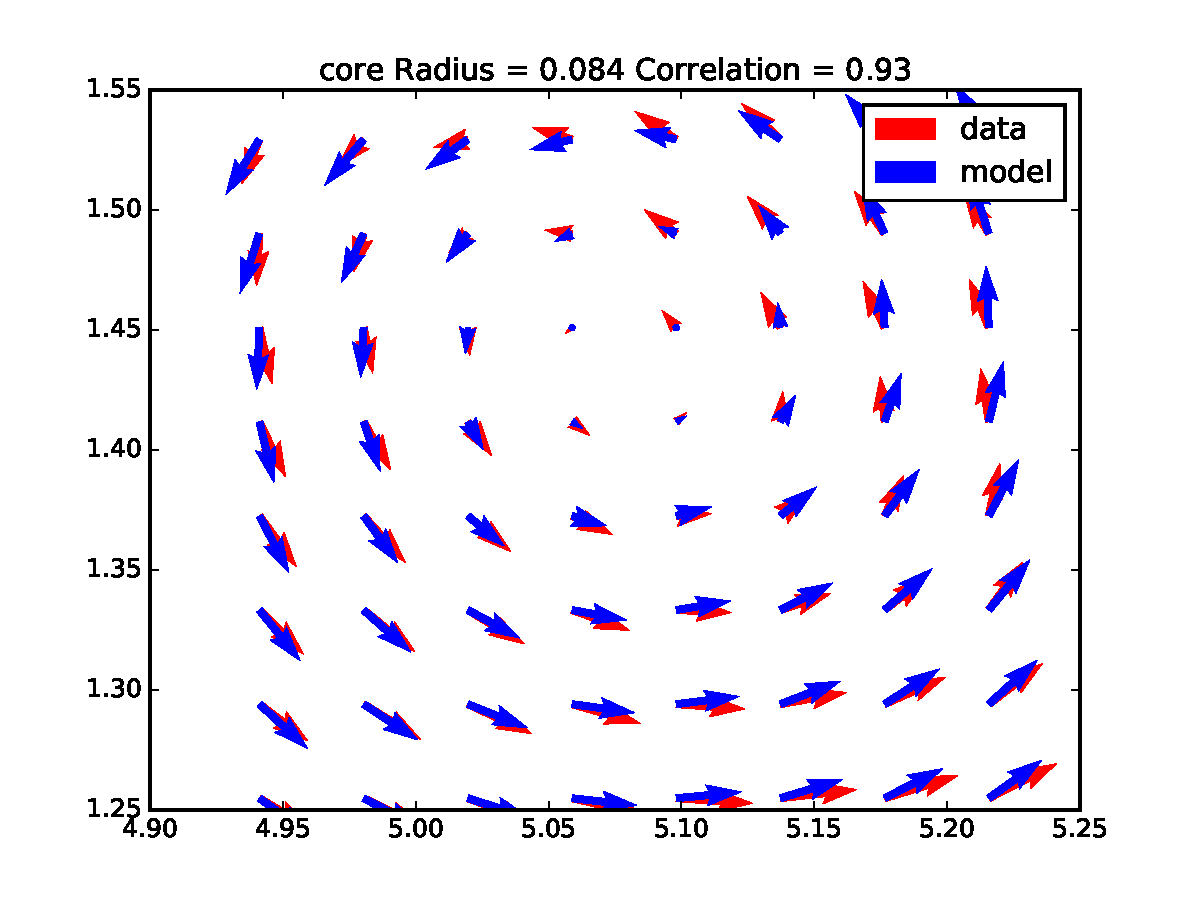
\includegraphics[trim=40 20 40 20 ,clip, width=\textwidth]{figure/dns_fit3.pdf}
		\caption{}
	\end{subfigure}
	\begin{subfigure}[b]{0.45\textwidth}
		\centering
		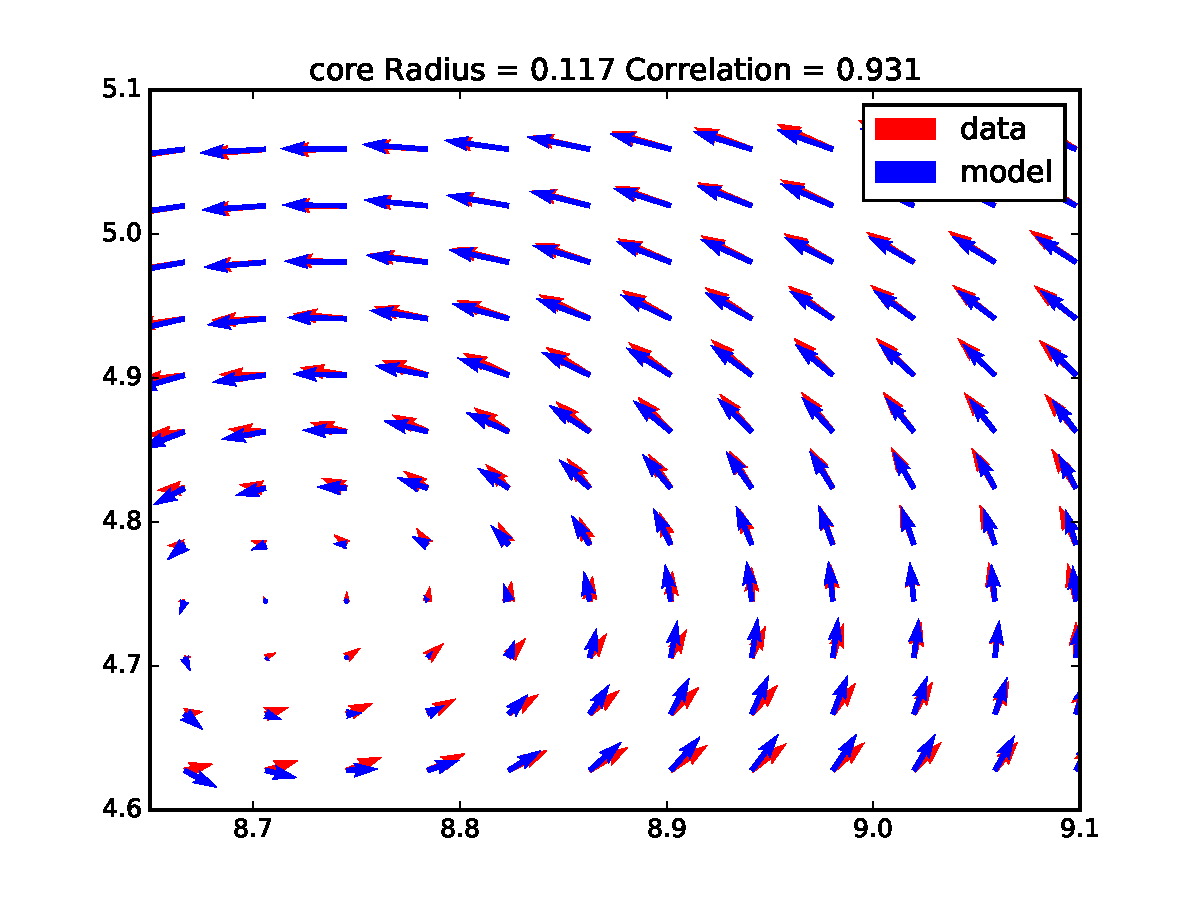
\includegraphics[trim=40 20 40 20 ,clip, width=\textwidth]{figure/dns_fit6.pdf}
		\caption{}
	\end{subfigure}
	\caption{Velocity vectors of fitted vortices from HIT DNS data}
	\label{fig:vorticesDNS}
\end{figure}

Figure \ref{fig:vorticesDNS} shows 4 random fitted vortices from the DNS, and table \ref{tb:DNSvortices} describes its characteristics.

\begin{table}[h!]
	\centering
	\caption{Characteristics of 4 random vortices from HIT DNS data}
	\vspace{10px}
	\label{tb:DNSvortices}
	\begin{tabular}{c|c|c|c|c}
		 Center(x,y) & Radius    & $\Gamma$   & Correlation & Box window \\
		\hline
		 37, 50   & 0.1226  & 6.0498   & 0.7818 & 6 \\
		 93, 79   & 0.0745  & 7.9175   & 0.8590 & 4 \\
		 130, 36  & 0.0844  & -11.3036 & 0.9305 & 4\\
		 227, 124 & 0.11727 & -13.6144 & 0.9309 & 6
	\end{tabular}
\end{table}

\chapter{Conclusion}

In this project we have developed a program capable of detecting and fitting vortices using the Lamb-Oseen vortex model. Several options are available, like choosing the differencing scheme, detection method, boxsize of detection and the non linear least squares method. The modular design of the program allows to easily add more options to any of the steps of the process.

The detection methods, Q criterion, $\Delta$ criterion and Swirling Strength perform about the same on our procedure. The small difference is on the quantity of initially detected vortices, but after the fitting this small difference disappears as false-positive vortices.

The Levenberg Marquardt method and Powell's dogleg method tend to fit correctly the accepted vortices. One strength of the Powell's method is that we have a trusted region, that allows us to set bounds on the fitting procedure, preventing some unreal results where some parameters can increase more than four orders of magnitude.

Currently we have a well tuned program for the HIT case, and as a future work a better approach to the PIV data will be added.   

%\section{PIV data}

%\begin{figure}[h]
%	\centering
%	\label{fig:detectionPIV}
%	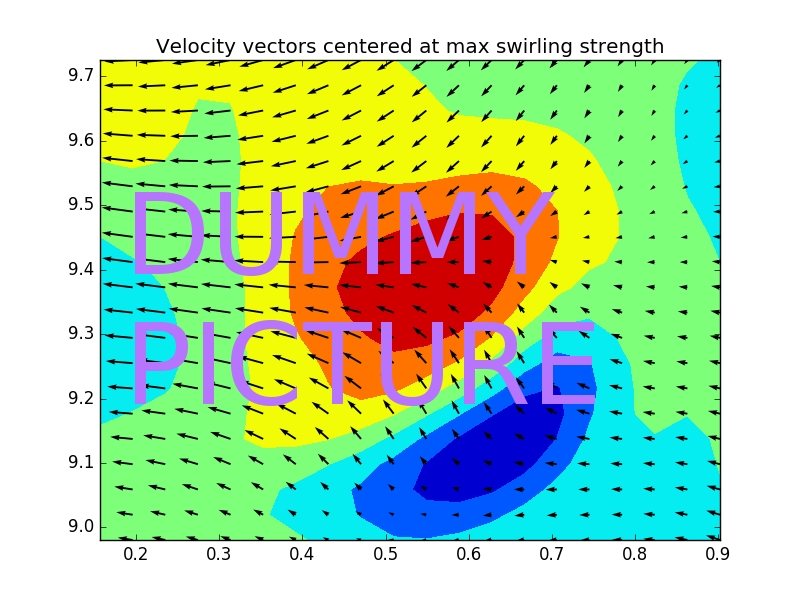
\includegraphics[scale=0.5]{figure/dummy.png}
%	\caption{Detected vortices from the PIV data}
%\end{figure}

\newpage
\bibliographystyle{plain}
\bibliography{biblio}

\appendix

\chapter{Finite difference methods}

\section{Second order accurate}
\label{annex:finite}
Two schemes were selected to be implemented, the 2nd order scheme and the 4th order scheme. The stencils are presented below.

Second order central differencing scheme, on interior cells:
\begin{equation}
F_x(i) = \frac{F(i+1)-F(i-1)}{2 \Delta x}
\end{equation}

Forward at left edge cells:
\begin{equation}
F_x(i) = \frac{F(i+1)-F(i)}{\Delta x}
\end{equation}

Backward at right edge cells:
\begin{equation}
F_x(n) = \frac{F(n)-F(n-1)}{\Delta x}
\end{equation}

\section{Fourth order accurate}

\begin{equation}
F_x(i) = \frac{-F(i+2)+8F(i+1)-8F(i-1)+F(i-2)}{12 \Delta x}
\end{equation}

left edge cells:
\begin{equation}
F_x(i) = \frac{F(i+3)-6F(i+2)+18F(i+1)-10F(i) -3F(i-1)}{12 \Delta x}
\end{equation}

right edge cells:
\begin{equation}
F_x(i) = \frac{3F(i+1)+10F(i)-18F(i-1)+6F(i-2) -F(i-3)}{12 \Delta x}
\end{equation}

\chapter{Python Code}
Here we have the main parts of the program developed in Python, vortexFitting, detection and fitting.

\section{vortexFitting.py}

\lstinputlisting[language=Python,basicstyle=\ttm,otherkeywords={self},keywordstyle=\ttb\color{deepblue},
emph={__init__},emphstyle=\ttb\color{deepred},stringstyle=\color{deepgreen},frame=tb,showstringspaces=false]
{/home/guilherme/Documents/VortexFitting/docs/report/vortexfitting.py}

\section{detection.py}

\lstinputlisting[language=Python,basicstyle=\ttm,otherkeywords={self},keywordstyle=\ttb\color{deepblue},
emph={__init__},emphstyle=\ttb\color{deepred},stringstyle=\color{deepgreen},frame=tb,showstringspaces=false]
{/home/guilherme/Documents/VortexFitting/docs/report/detection.py}

\section{fitting.py}

\lstinputlisting[language=Python,basicstyle=\ttm,otherkeywords={self},keywordstyle=\ttb\color{deepblue},
emph={__init__},emphstyle=\ttb\color{deepred},stringstyle=\color{deepgreen},frame=tb,showstringspaces=false]
{/home/guilherme/Documents/VortexFitting/docs/report/fitting.py}


\end{document}














